
\documentclass[preprint,12pt]{elsarticle}

\usepackage[spanish]{babel}
\usepackage{amssymb}
\usepackage{graphicx}
\usepackage{lineno}
\usepackage[utf8]{inputenc}
\usepackage{url}
\usepackage{natbib} 
\usepackage{amsmath} 
\usepackage{amssymb} 

\begin{document}
	
	\begin{frontmatter} 

		\title{\huge MESA DE AYUDA}
		
		\author{Huichi Contreras, Franklin Carlos            (2016056193)}
		\author{Gonzales Cave, Angel Gabriel              	(2017057861)}
		\author{Condori Quispe, Yhónn Joel	         	(2016056358)} 
		\author{Pastor Mendoza, José Edilberto             	(2016055237)} 
		\address{Escuela Profesional de Ingeniería de Sistemas}
		\address{Universidad Privada de Tacna}
		\address{Tacna, Perú}
		
%% ABSTRACT --------------------------------------------------------------------------------------------------------------------

		\begin{abstract}
		


		\end{abstract}

%% ----------------------------------------------------------------------------------------------------------------------------------

	\end{frontmatter}

%% RESUMEN ---------------------------------------------------------------------------------------------------------------------

\section{Resumen}



%% ----------------------------------------------------------------------------------------------------------------------------------


%% INTRODUCION ----------------------------------------------------------------------------------------------------------------

\section{Introducción} 

EDITAR\\

%% ----------------------------------------------------------------------------------------------------------------------------------


%% TITULO  ------------------------------------------------------------------------------------------------------------

\section{Titulo}

EDITAR\\

%% ----------------------------------------------------------------------------------------------------------------------------------

%% AUTORES  ------------------------------------------------------------------------------------------------------------

\section{Autores}

EDITAR\\

%% ----------------------------------------------------------------------------------------------------------------------------------

%% PLANTEAMIENTO DEL PROBLEMA ------------------------------------------------------------------------------------------------------------

\section{Planteamiento del problema}

%%  SUBSECCION 

\subsection {\textbf{Problema}}

EDITAR\\

%%  SUBSECCION 

\subsection {\textbf{Justificacion}}

EDITAR\\

%%Ejemplo de cita
\cite{Gartner} 

\begin{itemize}
	\item x
	\item y
	\item z
\end{itemize}

%%  SUBSECCION 

\subsection {\textbf{Alcance}}

EDITAR\\

%% ----------------------------------------------------------------------------------------------------------------------------------

%% OBJETIVOS ------------------------------------------------------------------------------------------------------------

\section{Objetivos}

EDITAR\\

%% Ejemplo de inclusión de imagen
\begin{figure}[htb]
	\begin{center}
		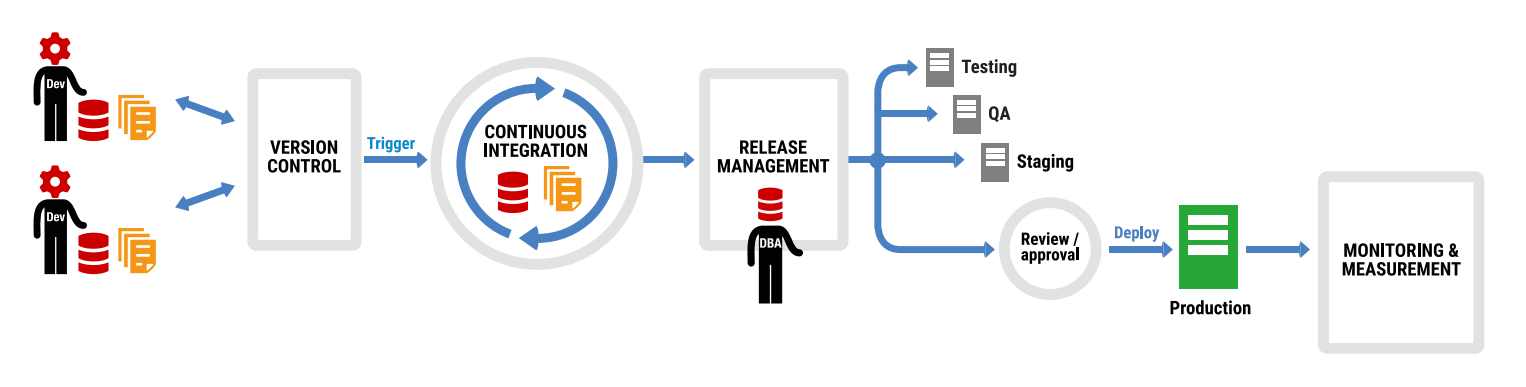
\includegraphics[width=14cm]{./IMAGENES/basededatos_1} 
		\caption{Incluyendo la base de datos en DevOps}
	\end{center}
\end{figure}

%%  SUBSECCION 

\subsection{\textbf{General}}

EDITAR\\

\begin{itemize}

\item x
\item y
\item z

\end{itemize}

%%  SUBSECCION 

\subsection{\textbf{Especificos}}

EDITAR\\

%% ----------------------------------------------------------------------------------------------------------------------------------
 

%% REFERENTES TEORICOS ---------------------------------------------------------------------------------------------------

\section{Referentes Teoricos}

EDITAR\\

%% ----------------------------------------------------------------------------------------------------------------------------------


%% DESARROLLO DE LA PROPUESTA ---------------------------------------------------------------------------------------------------

\section{Desarrollo de la propuesta}

EDITAR\\

%%  SUBSECCION 

\subsection{\textbf{Tecnología de información}}

EDITAR\\

%%  SUBSECCION 

\subsection{\textbf{Metodología, técnicas usadas}}

EDITAR\\

%% ----------------------------------------------------------------------------------------------------------------------------------

%% CRONOGRAMA (PERSONAS, TIEMPO, OTROS RECURSOS) ---------------------------------------------------------------------------------------------------

\section{Cronograma}

EDITAR\\

%% ----------------------------------------------------------------------------------------------------------------------------------



%%  REFERENCIAS BIBLIOGRÁFICAS  (OJO NO TOCAR CON CITEP SOLO SE PONEN)------------------------------------------------------------------------------------------
	
	\newpage
	
	\bibliographystyle{apalike} 	%ESTILO
	\bibliography{BIBLIOGRAFIA}	 
	
	
\end{document}
